% GNUPLOT: LaTeX picture with Postscript
\documentclass{minimal}
% Set font size
\makeatletter
\def\@ptsize{1}
\InputIfFileExists{size11.clo}{}{%
   \GenericError{(gnuplot) \space\space\space\@spaces}{%
      Gnuplot Error: File `size11.clo' not found! Could not set font size%
   }{See the gnuplot documentation for explanation.%
   }{For using a font size a file `size<fontsize>.clo' has to exist.
        Falling back ^^Jto default fontsize 10pt.}%
  \def\@ptsize{0}
  \input{size10.clo}%
}%
\makeatother
% Load packages
\usepackage{calc}
\usepackage{graphicx}
\usepackage{color}
\usepackage{transparent}
\makeatletter
% Select an appropriate default driver (from TeXLive graphics.cfg)
\begingroup
  \chardef\x=0 %
  % check pdfTeX
  \@ifundefined{pdfoutput}{}{%
    \ifcase\pdfoutput
    \else
      \chardef\x=1 %
    \fi
  }%
  % check VTeX
  \@ifundefined{OpMode}{}{%
    \chardef\x=2 %
  }%
\expandafter\endgroup
\ifcase\x
  % default case
  \PassOptionsToPackage{dvips}{geometry}
\or
  % pdfTeX is running in pdf mode
  \PassOptionsToPackage{pdftex}{geometry}
\else
  % VTeX is running
  \PassOptionsToPackage{vtex}{geometry}
\fi
\makeatother
% Set papersize
\usepackage[papersize={850.00bp,566.00bp},text={850.00bp,566.00bp}]{geometry}
% No page numbers and no paragraph indentation
\pagestyle{empty}
\setlength{\parindent}{0bp}%
% Load configuration file
\InputIfFileExists{gnuplot.cfg}{%
  \typeout{Using configuration file gnuplot.cfg}%
}{%
 \typeout{No configuration file gnuplot.cfg found.}%
}%
%
\begin{document}
\begingroup
  \makeatletter
  \providecommand\color[2][]{%
    \GenericError{(gnuplot) \space\space\space\@spaces}{%
      Package color not loaded in conjunction with
      terminal option `colourtext'%
    }{See the gnuplot documentation for explanation.%
    }{Either use 'blacktext' in gnuplot or load the package
      color.sty in LaTeX.}%
    \renewcommand\color[2][]{}%
  }%
  \providecommand\includegraphics[2][]{%
    \GenericError{(gnuplot) \space\space\space\@spaces}{%
      Package graphicx or graphics not loaded%
    }{See the gnuplot documentation for explanation.%
    }{The gnuplot epslatex terminal needs graphicx.sty or graphics.sty.}%
    \renewcommand\includegraphics[2][]{}%
  }%
  \providecommand\rotatebox[2]{#2}%
  \@ifundefined{ifGPcolor}{%
    \newif\ifGPcolor
    \GPcolortrue
  }{}%
  \@ifundefined{ifGPblacktext}{%
    \newif\ifGPblacktext
    \GPblacktextfalse
  }{}%
  % define a \g@addto@macro without @ in the name:
  \let\gplgaddtomacro\g@addto@macro
  % define empty templates for all commands taking text:
  \gdef\gplbacktext{}%
  \gdef\gplfronttext{}%
  \makeatother
  \ifGPblacktext
    % no textcolor at all
    \def\colorrgb#1{}%
    \def\colorgray#1{}%
  \else
    % gray or color?
    \ifGPcolor
      \def\colorrgb#1{\color[rgb]{#1}}%
      \def\colorgray#1{\color[gray]{#1}}%
      \expandafter\def\csname LTw\endcsname{\color{white}}%
      \expandafter\def\csname LTb\endcsname{\color{black}}%
      \expandafter\def\csname LTa\endcsname{\color{black}}%
      \expandafter\def\csname LT0\endcsname{\color[rgb]{1,0,0}}%
      \expandafter\def\csname LT1\endcsname{\color[rgb]{0,1,0}}%
      \expandafter\def\csname LT2\endcsname{\color[rgb]{0,0,1}}%
      \expandafter\def\csname LT3\endcsname{\color[rgb]{1,0,1}}%
      \expandafter\def\csname LT4\endcsname{\color[rgb]{0,1,1}}%
      \expandafter\def\csname LT5\endcsname{\color[rgb]{1,1,0}}%
      \expandafter\def\csname LT6\endcsname{\color[rgb]{0,0,0}}%
      \expandafter\def\csname LT7\endcsname{\color[rgb]{1,0.3,0}}%
      \expandafter\def\csname LT8\endcsname{\color[rgb]{0.5,0.5,0.5}}%
    \else
      % gray
      \def\colorrgb#1{\color{black}}%
      \def\colorgray#1{\color[gray]{#1}}%
      \expandafter\def\csname LTw\endcsname{\color{white}}%
      \expandafter\def\csname LTb\endcsname{\color{black}}%
      \expandafter\def\csname LTa\endcsname{\color{black}}%
      \expandafter\def\csname LT0\endcsname{\color{black}}%
      \expandafter\def\csname LT1\endcsname{\color{black}}%
      \expandafter\def\csname LT2\endcsname{\color{black}}%
      \expandafter\def\csname LT3\endcsname{\color{black}}%
      \expandafter\def\csname LT4\endcsname{\color{black}}%
      \expandafter\def\csname LT5\endcsname{\color{black}}%
      \expandafter\def\csname LT6\endcsname{\color{black}}%
      \expandafter\def\csname LT7\endcsname{\color{black}}%
      \expandafter\def\csname LT8\endcsname{\color{black}}%
    \fi
  \fi
    \setlength{\unitlength}{0.0500bp}%
    \ifx\gptboxheight\undefined%
      \newlength{\gptboxheight}%
      \newlength{\gptboxwidth}%
      \newsavebox{\gptboxtext}%
    \fi%
    \setlength{\fboxrule}{0.5pt}%
    \setlength{\fboxsep}{1pt}%
\begin{picture}(17000.00,11320.00)%
    \gplgaddtomacro\gplbacktext{%
      \csname LTb\endcsname%%
      \put(561,6595){\makebox(0,0)[r]{\strut{}$-2$}}%
      \csname LTb\endcsname%%
      \put(561,7318){\makebox(0,0)[r]{\strut{}$0$}}%
      \csname LTb\endcsname%%
      \put(561,8041){\makebox(0,0)[r]{\strut{}$2$}}%
      \csname LTb\endcsname%%
      \put(561,8763){\makebox(0,0)[r]{\strut{}$4$}}%
      \csname LTb\endcsname%%
      \put(561,9486){\makebox(0,0)[r]{\strut{}$6$}}%
      \csname LTb\endcsname%%
      \put(561,10208){\makebox(0,0)[r]{\strut{}$8$}}%
      \csname LTb\endcsname%%
      \put(561,10931){\makebox(0,0)[r]{\strut{}$10$}}%
      \csname LTb\endcsname%%
      \put(1133,6048){\makebox(0,0){\strut{}$-4$}}%
      \csname LTb\endcsname%%
      \put(2072,6048){\makebox(0,0){\strut{}$-2$}}%
      \csname LTb\endcsname%%
      \put(3012,6048){\makebox(0,0){\strut{}$0$}}%
      \csname LTb\endcsname%%
      \put(3951,6048){\makebox(0,0){\strut{}$2$}}%
      \csname LTb\endcsname%%
      \put(4890,6048){\makebox(0,0){\strut{}$4$}}%
      \csname LTb\endcsname%%
      \put(898,10461){\makebox(0,0)[l]{\strut{}\Huge $x^{2}$}}%
    }%
    \gplgaddtomacro\gplfronttext{%
      \csname LTb\endcsname%%
      \put(153,8582){\makebox(0,0){\strut{}\Huge$y$}}%
    }%
    \gplgaddtomacro\gplbacktext{%
      \csname LTb\endcsname%%
      \put(6023,6622){\makebox(0,0)[r]{\strut{}$-4$}}%
      \csname LTb\endcsname%%
      \put(6023,7602){\makebox(0,0)[r]{\strut{}$-2$}}%
      \csname LTb\endcsname%%
      \put(6023,8583){\makebox(0,0)[r]{\strut{}$0$}}%
      \csname LTb\endcsname%%
      \put(6023,9563){\makebox(0,0)[r]{\strut{}$2$}}%
      \csname LTb\endcsname%%
      \put(6023,10543){\makebox(0,0)[r]{\strut{}$4$}}%
      \csname LTb\endcsname%%
      \put(6125,5946){\makebox(0,0){\strut{}$-3$}}%
      \csname LTb\endcsname%%
      \put(6942,5946){\makebox(0,0){\strut{}$-2$}}%
      \csname LTb\endcsname%%
      \put(7759,5946){\makebox(0,0){\strut{}$-1$}}%
      \csname LTb\endcsname%%
      \put(8576,5946){\makebox(0,0){\strut{}$0$}}%
      \csname LTb\endcsname%%
      \put(9392,5946){\makebox(0,0){\strut{}$1$}}%
      \csname LTb\endcsname%%
      \put(10209,5946){\makebox(0,0){\strut{}$2$}}%
      \csname LTb\endcsname%%
      \put(11026,5946){\makebox(0,0){\strut{}$3$}}%
      \csname LTb\endcsname%%
      \put(6370,10543){\makebox(0,0)[l]{\strut{}\Huge $x^{3}$}}%
    }%
    \gplgaddtomacro\gplfronttext{%
    }%
    \gplgaddtomacro\gplbacktext{%
      \csname LTb\endcsname%%
      \put(11690,6132){\makebox(0,0)[r]{\strut{}$-4$}}%
      \csname LTb\endcsname%%
      \put(11690,6745){\makebox(0,0)[r]{\strut{}$-3$}}%
      \csname LTb\endcsname%%
      \put(11690,7357){\makebox(0,0)[r]{\strut{}$-2$}}%
      \csname LTb\endcsname%%
      \put(11690,7970){\makebox(0,0)[r]{\strut{}$-1$}}%
      \csname LTb\endcsname%%
      \put(11690,8583){\makebox(0,0)[r]{\strut{}$0$}}%
      \csname LTb\endcsname%%
      \put(11690,9195){\makebox(0,0)[r]{\strut{}$1$}}%
      \csname LTb\endcsname%%
      \put(11690,9808){\makebox(0,0)[r]{\strut{}$2$}}%
      \csname LTb\endcsname%%
      \put(11690,10420){\makebox(0,0)[r]{\strut{}$3$}}%
      \csname LTb\endcsname%%
      \put(11690,11033){\makebox(0,0)[r]{\strut{}$4$}}%
      \csname LTb\endcsname%%
      \put(11792,5946){\makebox(0,0){\strut{}$-15$}}%
      \csname LTb\endcsname%%
      \put(12609,5946){\makebox(0,0){\strut{}$-10$}}%
      \csname LTb\endcsname%%
      \put(13426,5946){\makebox(0,0){\strut{}$-5$}}%
      \csname LTb\endcsname%%
      \put(14243,5946){\makebox(0,0){\strut{}$0$}}%
      \csname LTb\endcsname%%
      \put(15059,5946){\makebox(0,0){\strut{}$5$}}%
      \csname LTb\endcsname%%
      \put(15876,5946){\makebox(0,0){\strut{}$10$}}%
      \csname LTb\endcsname%%
      \put(16693,5946){\makebox(0,0){\strut{}$15$}}%
      \csname LTb\endcsname%%
      \put(12037,10543){\makebox(0,0)[l]{\strut{}\Huge $\sin\left(x\right)$}}%
    }%
    \gplgaddtomacro\gplfronttext{%
    }%
    \gplgaddtomacro\gplbacktext{%
      \csname LTb\endcsname%%
      \put(561,686){\makebox(0,0)[r]{\strut{}$-4$}}%
      \csname LTb\endcsname%%
      \put(561,1273){\makebox(0,0)[r]{\strut{}$-3$}}%
      \csname LTb\endcsname%%
      \put(561,1860){\makebox(0,0)[r]{\strut{}$-2$}}%
      \csname LTb\endcsname%%
      \put(561,2447){\makebox(0,0)[r]{\strut{}$-1$}}%
      \csname LTb\endcsname%%
      \put(561,3035){\makebox(0,0)[r]{\strut{}$0$}}%
      \csname LTb\endcsname%%
      \put(561,3622){\makebox(0,0)[r]{\strut{}$1$}}%
      \csname LTb\endcsname%%
      \put(561,4209){\makebox(0,0)[r]{\strut{}$2$}}%
      \csname LTb\endcsname%%
      \put(561,4796){\makebox(0,0)[r]{\strut{}$3$}}%
      \csname LTb\endcsname%%
      \put(561,5383){\makebox(0,0)[r]{\strut{}$4$}}%
      \csname LTb\endcsname%%
      \put(825,500){\makebox(0,0){\strut{}$-4$}}%
      \csname LTb\endcsname%%
      \put(1473,500){\makebox(0,0){\strut{}$-2$}}%
      \csname LTb\endcsname%%
      \put(2121,500){\makebox(0,0){\strut{}$0$}}%
      \csname LTb\endcsname%%
      \put(2769,500){\makebox(0,0){\strut{}$2$}}%
      \csname LTb\endcsname%%
      \put(3416,500){\makebox(0,0){\strut{}$4$}}%
      \csname LTb\endcsname%%
      \put(4064,500){\makebox(0,0){\strut{}$6$}}%
      \csname LTb\endcsname%%
      \put(4712,500){\makebox(0,0){\strut{}$8$}}%
      \csname LTb\endcsname%%
      \put(5360,500){\makebox(0,0){\strut{}$10$}}%
      \csname LTb\endcsname%%
      \put(757,4913){\makebox(0,0)[l]{\strut{}\Huge $\log\left(x\right)$}}%
    }%
    \gplgaddtomacro\gplfronttext{%
      \csname LTb\endcsname%%
      \put(153,3034){\makebox(0,0){\strut{}\Huge$y$}}%
      \csname LTb\endcsname%%
      \put(3011,221){\makebox(0,0){\strut{}\Huge$x$}}%
    }%
    \gplgaddtomacro\gplbacktext{%
      \csname LTb\endcsname%%
      \put(6034,595){\makebox(0,0)[r]{\strut{}$-1$}}%
      \csname LTb\endcsname%%
      \put(6034,1571){\makebox(0,0)[r]{\strut{}$0$}}%
      \csname LTb\endcsname%%
      \put(6034,2547){\makebox(0,0)[r]{\strut{}$1$}}%
      \csname LTb\endcsname%%
      \put(6034,3522){\makebox(0,0)[r]{\strut{}$2$}}%
      \csname LTb\endcsname%%
      \put(6034,4498){\makebox(0,0)[r]{\strut{}$3$}}%
      \csname LTb\endcsname%%
      \put(6034,5474){\makebox(0,0)[r]{\strut{}$4$}}%
      \csname LTb\endcsname%%
      \put(6136,409){\makebox(0,0){\strut{}$-6$}}%
      \csname LTb\endcsname%%
      \put(6949,409){\makebox(0,0){\strut{}$-4$}}%
      \csname LTb\endcsname%%
      \put(7762,409){\makebox(0,0){\strut{}$-2$}}%
      \csname LTb\endcsname%%
      \put(8576,409){\makebox(0,0){\strut{}$0$}}%
      \csname LTb\endcsname%%
      \put(9389,409){\makebox(0,0){\strut{}$2$}}%
      \csname LTb\endcsname%%
      \put(10202,409){\makebox(0,0){\strut{}$4$}}%
      \csname LTb\endcsname%%
      \put(11015,409){\makebox(0,0){\strut{}$6$}}%
      \csname LTb\endcsname%%
      \put(6380,4986){\makebox(0,0)[l]{\strut{}\Huge $\left|x\right|$}}%
    }%
    \gplgaddtomacro\gplfronttext{%
      \csname LTb\endcsname%%
      \put(8575,130){\makebox(0,0){\strut{}\Huge$x$}}%
    }%
    \gplgaddtomacro\gplbacktext{%
      \csname LTb\endcsname%%
      \put(11701,595){\makebox(0,0)[r]{\strut{}$-1$}}%
      \csname LTb\endcsname%%
      \put(11701,1408){\makebox(0,0)[r]{\strut{}$0$}}%
      \csname LTb\endcsname%%
      \put(11701,2221){\makebox(0,0)[r]{\strut{}$1$}}%
      \csname LTb\endcsname%%
      \put(11701,3035){\makebox(0,0)[r]{\strut{}$2$}}%
      \csname LTb\endcsname%%
      \put(11701,3848){\makebox(0,0)[r]{\strut{}$3$}}%
      \csname LTb\endcsname%%
      \put(11701,4661){\makebox(0,0)[r]{\strut{}$4$}}%
      \csname LTb\endcsname%%
      \put(11701,5474){\makebox(0,0)[r]{\strut{}$5$}}%
      \csname LTb\endcsname%%
      \put(12178,409){\makebox(0,0){\strut{}$-2$}}%
      \csname LTb\endcsname%%
      \put(12929,409){\makebox(0,0){\strut{}$0$}}%
      \csname LTb\endcsname%%
      \put(13680,409){\makebox(0,0){\strut{}$2$}}%
      \csname LTb\endcsname%%
      \put(14430,409){\makebox(0,0){\strut{}$4$}}%
      \csname LTb\endcsname%%
      \put(15181,409){\makebox(0,0){\strut{}$6$}}%
      \csname LTb\endcsname%%
      \put(15931,409){\makebox(0,0){\strut{}$8$}}%
      \csname LTb\endcsname%%
      \put(16682,409){\makebox(0,0){\strut{}$10$}}%
      \csname LTb\endcsname%%
      \put(12047,4986){\makebox(0,0)[l]{\strut{}\Huge $\sqrt{x}$}}%
    }%
    \gplgaddtomacro\gplfronttext{%
      \csname LTb\endcsname%%
      \put(14242,130){\makebox(0,0){\strut{}\Huge$x$}}%
    }%
    \gplbacktext
    \put(0,0){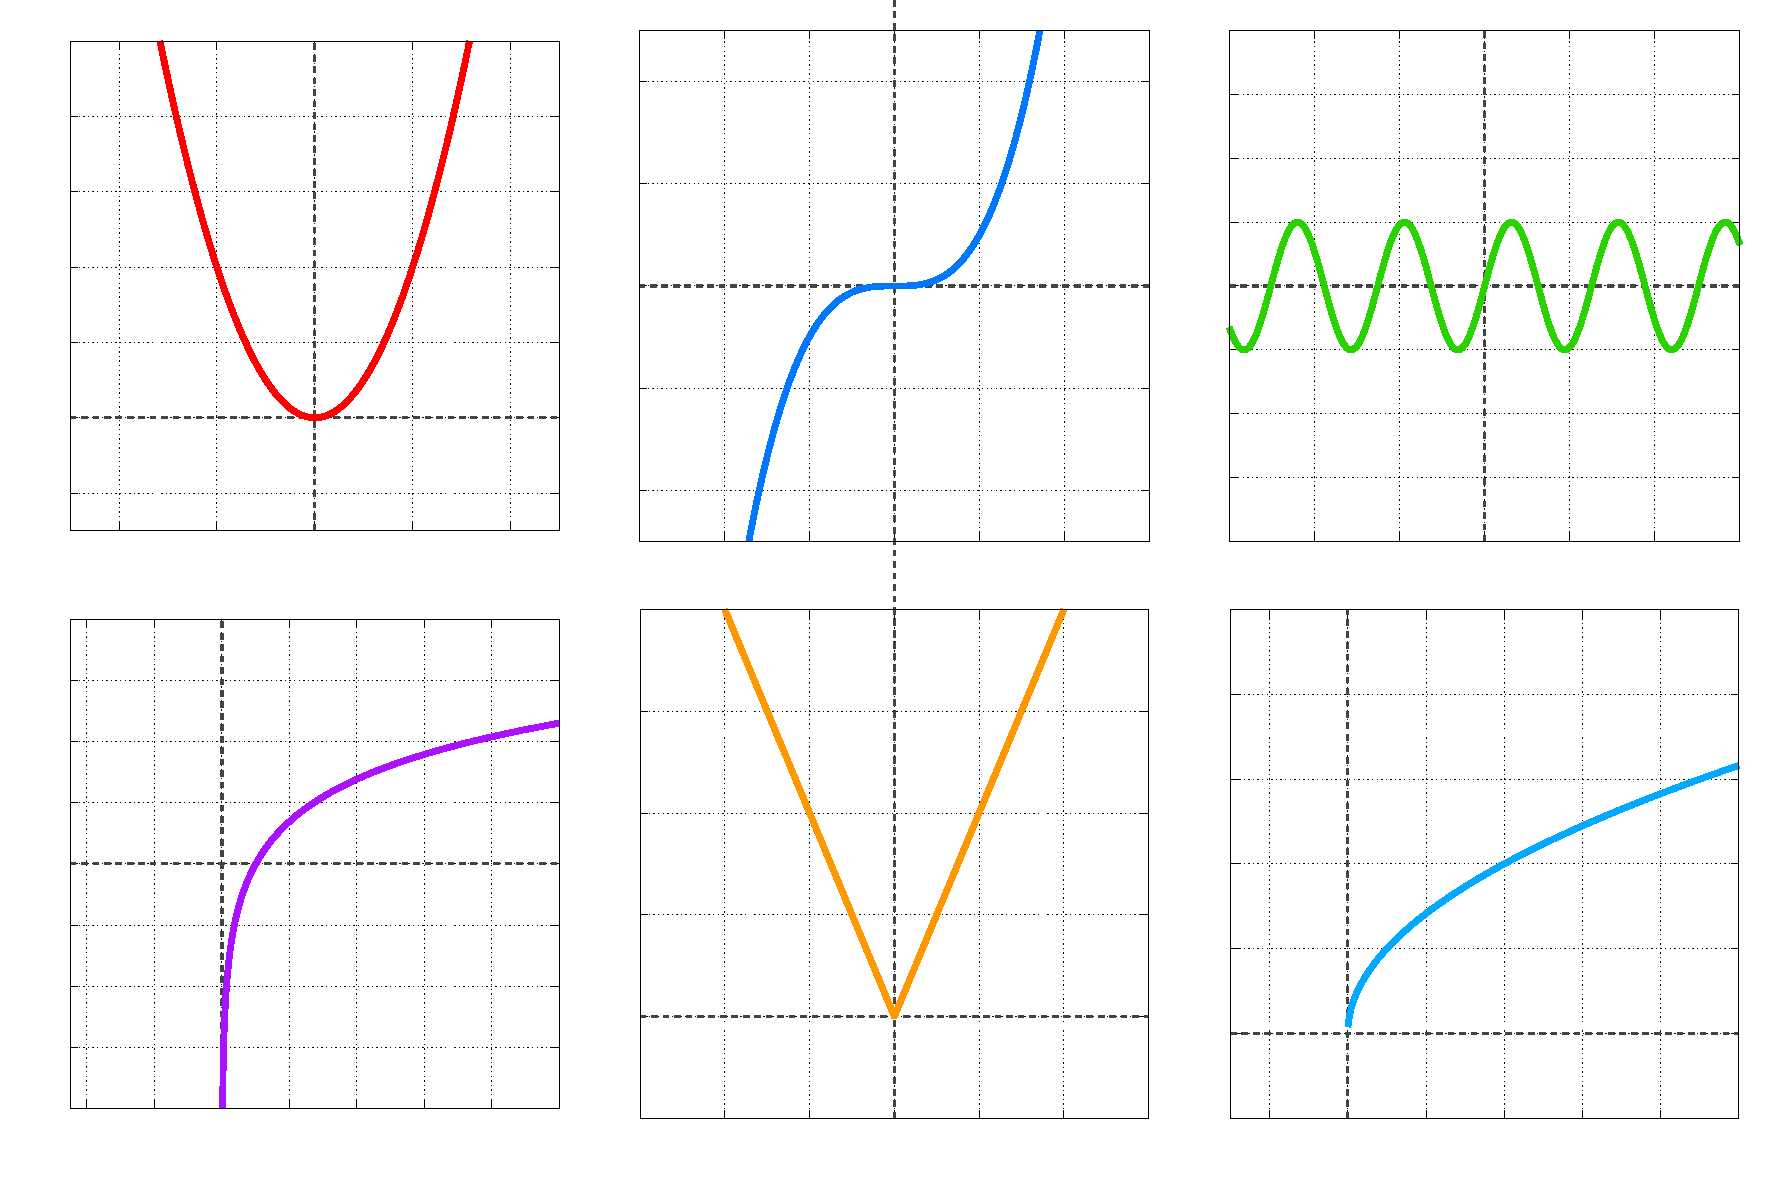
\includegraphics{func_graphs-inc}}%
    \gplfronttext
  \end{picture}%
\endgroup
\end{document}
